
%% bare_jrnl_transmag.tex
%% V1.4a
%% 2014/09/17
%% by Michael Shell
%% see http://www.michaelshell.org/
%% for current contact information.
%%
%% This is a skeleton file demonstrating the use of IEEEtran.cls
%% (requires IEEEtran.cls version 1.8a or later) with an IEEE 
%% Transactions on Magnetics journal paper.
%%
%% Support sites:
%% http://www.michaelshell.org/tex/ieeetran/
%% http://www.ctan.org/tex-archive/macros/latex/contrib/IEEEtran/
%% and
%% http://www.ieee.org/

%%*************************************************************************
%% Legal Notice:
%% This code is offered as-is without any warranty either expressed or
%% implied; without even the implied warranty of MERCHANTABILITY or
%% FITNESS FOR A PARTICULAR PURPOSE! 
%% User assumes all risk.
%% In no event shall IEEE or any contributor to this code be liable for
%% any damages or losses, including, but not limited to, incidental,
%% consequential, or any other damages, resulting from the use or misuse
%% of any information contained here.
%%
%% All comments are the opinions of their respective authors and are not
%% necessarily endorsed by the IEEE.
%%
%% This work is distributed under the LaTeX Project Public License (LPPL)
%% ( http://www.latex-project.org/ ) version 1.3, and may be freely used,
%% distributed and modified. A copy of the LPPL, version 1.3, is included
%% in the base LaTeX documentation of all distributions of LaTeX released
%% 2003/12/01 or later.
%% Retain all contribution notices and credits.
%% ** Modified files should be clearly indicated as such, including  **
%% ** renaming them and changing author support contact information. **
%%
%% File list of work: IEEEtran.cls, IEEEtran_HOWTO.pdf, bare_adv.tex,
%%                    bare_conf.tex, bare_jrnl.tex, bare_conf_compsoc.tex,
%%                    bare_jrnl_compsoc.tex, bare_jrnl_transmag.tex
%%*************************************************************************


% *** Authors should verify (and, if needed, correct) their LaTeX system  ***
% *** with the testflow diagnostic prior to trusting their LaTeX platform ***
% *** with production work. IEEE's font choices and paper sizes can       ***
% *** trigger bugs that do not appear when using other class files.       ***                          ***
% The testflow support page is at:
% http://www.michaelshell.org/tex/testflow/



\documentclass[journal,transmag,twoside]{IEEEtran}
%
% If IEEEtran.cls has not been installed into the LaTeX system files,
% manually specify the path to it like:
% \documentclass[journal]{../sty/IEEEtran}





% Some very useful LaTeX packages include:
% (uncomment the ones you want to load)


% *** MISC UTILITY PACKAGES ***
%
%\usepackage{ifpdf}
% Heiko Oberdiek's ifpdf.sty is very useful if you need conditional
% compilation based on whether the output is pdf or dvi.
% usage:
% \ifpdf
%   % pdf code
% \else
%   % dvi code
% \fi
% The latest version of ifpdf.sty can be obtained from:
% http://www.ctan.org/tex-archive/macros/latex/contrib/oberdiek/
% Also, note that IEEEtran.cls V1.7 and later provides a builtin
% \ifCLASSINFOpdf conditional that works the same way.
% When switching from latex to pdflatex and vice-versa, the compiler may
% have to be run twice to clear warning/error messages.






% *** CITATION PACKAGES ***
%
%\usepackage{cite}
% cite.sty was written by Donald Arseneau
% V1.6 and later of IEEEtran pre-defines the format of the cite.sty package
% \cite{} output to follow that of IEEE. Loading the cite package will
% result in citation numbers being automatically sorted and properly
% "compressed/ranged". e.g., [1], [9], [2], [7], [5], [6] without using
% cite.sty will become [1], [2], [5]--[7], [9] using cite.sty. cite.sty's
% \cite will automatically add leading space, if needed. Use cite.sty's
% noadjust option (cite.sty V3.8 and later) if you want to turn this off
% such as if a citation ever needs to be enclosed in parenthesis.
% cite.sty is already installed on most LaTeX systems. Be sure and use
% version 5.0 (2009-03-20) and later if using hyperref.sty.
% The latest version can be obtained at:
% http://www.ctan.org/tex-archive/macros/latex/contrib/cite/
% The documentation is contained in the cite.sty file itself.






% *** GRAPHICS RELATED PACKAGES ***
%
\ifCLASSINFOpdf
  \usepackage[pdftex]{graphicx}
  % declare the path(s) where your graphic files are
  % \graphicspath{{../pdf/}{../jpeg/}}
  % and their extensions so you won't have to specify these with
  % every instance of \includegraphics
  % \DeclareGraphicsExtensions{.pdf,.jpeg,.png}
\else
  % or other class option (dvipsone, dvipdf, if not using dvips). graphicx
  % will default to the driver specified in the system graphics.cfg if no
  % driver is specified.
  % \usepackage[dvips]{graphicx}
  % declare the path(s) where your graphic files are
  % \graphicspath{{../eps/}}
  % and their extensions so you won't have to specify these with
  % every instance of \includegraphics
  % \DeclareGraphicsExtensions{.eps}
\fi
% graphicx was written by David Carlisle and Sebastian Rahtz. It is
% required if you want graphics, photos, etc. graphicx.sty is already
% installed on most LaTeX systems. The latest version and documentation
% can be obtained at: 
% http://www.ctan.org/tex-archive/macros/latex/required/graphics/
% Another good source of documentation is "Using Imported Graphics in
% LaTeX2e" by Keith Reckdahl which can be found at:
% http://www.ctan.org/tex-archive/info/epslatex/
%
% latex, and pdflatex in dvi mode, support graphics in encapsulated
% postscript (.eps) format. pdflatex in pdf mode supports graphics
% in .pdf, .jpeg, .png and .mps (metapost) formats. Users should ensure
% that all non-photo figures use a vector format (.eps, .pdf, .mps) and
% not a bitmapped formats (.jpeg, .png). IEEE frowns on bitmapped formats
% which can result in "jaggedy"/blurry rendering of lines and letters as
% well as large increases in file sizes.
%
% You can find documentation about the pdfTeX application at:
% http://www.tug.org/applications/pdftex




% *** MATH PACKAGES ***
%
%\usepackage[cmex10]{amsmath}
% A popular package from the American Mathematical Society that provides
% many useful and powerful commands for dealing with mathematics. If using
% it, be sure to load this package with the cmex10 option to ensure that
% only type 1 fonts will utilized at all point sizes. Without this option,
% it is possible that some math symbols, particularly those within
% footnotes, will be rendered in bitmap form which will result in a
% document that can not be IEEE Xplore compliant!
%
% Also, note that the amsmath package sets \interdisplaylinepenalty to 10000
% thus preventing page breaks from occurring within multiline equations. Use:
%\interdisplaylinepenalty=2500
% after loading amsmath to restore such page breaks as IEEEtran.cls normally
% does. amsmath.sty is already installed on most LaTeX systems. The latest
% version and documentation can be obtained at:
% http://www.ctan.org/tex-archive/macros/latex/required/amslatex/math/





% *** SPECIALIZED LIST PACKAGES ***
%
%\usepackage{algorithmic}
% algorithmic.sty was written by Peter Williams and Rogerio Brito.
% This package provides an algorithmic environment fo describing algorithms.
% You can use the algorithmic environment in-text or within a figure
% environment to provide for a floating algorithm. Do NOT use the algorithm
% floating environment provided by algorithm.sty (by the same authors) or
% algorithm2e.sty (by Christophe Fiorio) as IEEE does not use dedicated
% algorithm float types and packages that provide these will not provide
% correct IEEE style captions. The latest version and documentation of
% algorithmic.sty can be obtained at:
% http://www.ctan.org/tex-archive/macros/latex/contrib/algorithms/
% There is also a support site at:
% http://algorithms.berlios.de/index.html
% Also of interest may be the (relatively newer and more customizable)
% algorithmicx.sty package by Szasz Janos:
% http://www.ctan.org/tex-archive/macros/latex/contrib/algorithmicx/




% *** ALIGNMENT PACKAGES ***
%
%\usepackage{array}
% Frank Mittelbach's and David Carlisle's array.sty patches and improves
% the standard LaTeX2e array and tabular environments to provide better
% appearance and additional user controls. As the default LaTeX2e table
% generation code is lacking to the point of almost being broken with
% respect to the quality of the end results, all users are strongly
% advised to use an enhanced (at the very least that provided by array.sty)
% set of table tools. array.sty is already installed on most systems. The
% latest version and documentation can be obtained at:
% http://www.ctan.org/tex-archive/macros/latex/required/tools/


% IEEEtran contains the IEEEeqnarray family of commands that can be used to
% generate multiline equations as well as matrices, tables, etc., of high
% quality.




% *** SUBFIGURE PACKAGES ***
%\ifCLASSOPTIONcompsoc
%  \usepackage[caption=false,font=normalsize,labelfont=sf,textfont=sf]{subfig}
%\else
%  \usepackage[caption=false,font=footnotesize]{subfig}
%\fi
% subfig.sty, written by Steven Douglas Cochran, is the modern replacement
% for subfigure.sty, the latter of which is no longer maintained and is
% incompatible with some LaTeX packages including fixltx2e. However,
% subfig.sty requires and automatically loads Axel Sommerfeldt's caption.sty
% which will override IEEEtran.cls' handling of captions and this will result
% in non-IEEE style figure/table captions. To prevent this problem, be sure
% and invoke subfig.sty's "caption=false" package option (available since
% subfig.sty version 1.3, 2005/06/28) as this is will preserve IEEEtran.cls
% handling of captions.
% Note that the Computer Society format requires a larger sans serif font
% than the serif footnote size font used in traditional IEEE formatting
% and thus the need to invoke different subfig.sty package options depending
% on whether compsoc mode has been enabled.
%
% The latest version and documentation of subfig.sty can be obtained at:
% http://www.ctan.org/tex-archive/macros/latex/contrib/subfig/



% *** FLOAT PACKAGES ***
%
%\usepackage{fixltx2e}
% fixltx2e, the successor to the earlier fix2col.sty, was written by
% Frank Mittelbach and David Carlisle. This package corrects a few problems
% in the LaTeX2e kernel, the most notable of which is that in current
% LaTeX2e releases, the ordering of single and double column floats is not
% guaranteed to be preserved. Thus, an unpatched LaTeX2e can allow a
% single column figure to be placed prior to an earlier double column
% figure. The latest version and documentation can be found at:
% http://www.ctan.org/tex-archive/macros/latex/base/


%\usepackage{stfloats}
% stfloats.sty was written by Sigitas Tolusis. This package gives LaTeX2e
% the ability to do double column floats at the bottom of the page as well
% as the top. (e.g., "\begin{figure*}[!b]" is not normally possible in
% LaTeX2e). It also provides a command:
%\fnbelowfloat
% to enable the placement of footnotes below bottom floats (the standard
% LaTeX2e kernel puts them above bottom floats). This is an invasive package
% which rewrites many portions of the LaTeX2e float routines. It may not work
% with other packages that modify the LaTeX2e float routines. The latest
% version and documentation can be obtained at:
% http://www.ctan.org/tex-archive/macros/latex/contrib/sttools/
% Do not use the stfloats baselinefloat ability as IEEE does not allow
% \baselineskip to stretch. Authors submitting work to the IEEE should note
% that IEEE rarely uses double column equations and that authors should try
% to avoid such use. Do not be tempted to use the cuted.sty or midfloat.sty
% packages (also by Sigitas Tolusis) as IEEE does not format its papers in
% such ways.
% Do not attempt to use stfloats with fixltx2e as they are incompatible.
% Instead, use Morten Hogholm'a dblfloatfix which combines the features
% of both fixltx2e and stfloats:
%
% \usepackage{dblfloatfix}
% The latest version can be found at:
% http://www.ctan.org/tex-archive/macros/latex/contrib/dblfloatfix/




%\ifCLASSOPTIONcaptionsoff
%  \usepackage[nomarkers]{endfloat}
% \let\MYoriglatexcaption\caption
% \renewcommand{\caption}[2][\relax]{\MYoriglatexcaption[#2]{#2}}
%\fi
% endfloat.sty was written by James Darrell McCauley, Jeff Goldberg and 
% Axel Sommerfeldt. This package may be useful when used in conjunction with 
% IEEEtran.cls'  captionsoff option. Some IEEE journals/societies require that
% submissions have lists of figures/tables at the end of the paper and that
% figures/tables without any captions are placed on a page by themselves at
% the end of the document. If needed, the draftcls IEEEtran class option or
% \CLASSINPUTbaselinestretch interface can be used to increase the line
% spacing as well. Be sure and use the nomarkers option of endfloat to
% prevent endfloat from "marking" where the figures would have been placed
% in the text. The two hack lines of code above are a slight modification of
% that suggested by in the endfloat docs (section 8.4.1) to ensure that
% the full captions always appear in the list of figures/tables - even if
% the user used the short optional argument of \caption[]{}.
% IEEE papers do not typically make use of \caption[]'s optional argument,
% so this should not be an issue. A similar trick can be used to disable
% captions of packages such as subfig.sty that lack options to turn off
% the subcaptions:
% For subfig.sty:
% \let\MYorigsubfloat\subfloat
% \renewcommand{\subfloat}[2][\relax]{\MYorigsubfloat[]{#2}}
% However, the above trick will not work if both optional arguments of
% the \subfloat command are used. Furthermore, there needs to be a
% description of each subfigure *somewhere* and endfloat does not add
% subfigure captions to its list of figures. Thus, the best approach is to
% avoid the use of subfigure captions (many IEEE journals avoid them anyway)
% and instead reference/explain all the subfigures within the main caption.
% The latest version of endfloat.sty and its documentation can obtained at:
% http://www.ctan.org/tex-archive/macros/latex/contrib/endfloat/
%
% The IEEEtran \ifCLASSOPTIONcaptionsoff conditional can also be used
% later in the document, say, to conditionally put the References on a 
% page by themselves.




% *** PDF, URL AND HYPERLINK PACKAGES ***
%
\usepackage{url}
% url.sty was written by Donald Arseneau. It provides better support for
% handling and breaking URLs. url.sty is already installed on most LaTeX
% systems. The latest version and documentation can be obtained at:
% http://www.ctan.org/tex-archive/macros/latex/contrib/url/
% Basically, \url{my_url_here}.

\usepackage{hyperref}
\newcommand{\email}[1]{\href{mailto:#1}{#1}}

\usepackage{pdfcomment}
\usepackage{xcolor}
\newcommand{\karrcomment}[2]{\pdfmarkupcomment[markup=Highlight,color=yellow,author={Jonathan Karr}]{#1}{#2}}


% *** Do not adjust lengths that control margins, column widths, etc. ***
% *** Do not use packages that alter fonts (such as pslatex).         ***
% There should be no need to do such things with IEEEtran.cls V1.6 and later.
% (Unless specifically asked to do so by the journal or conference you plan
% to submit to, of course. )

\usepackage{color,soul} % for highlighting only

%http://tex.stackexchange.com/questions/61265/why-doesnt-the-ieeetran-document-class-recognize-definition-environments
\newtheorem{definition}{Definition}

% correct bad hyphenation here
\hyphenation{op-tical net-works semi-conduc-tor}

% Nature News on irreproducibility:
% http://www.nature.com/news/reproducibility-1.17552

\begin{document}

\title{Engineering Dynamical Models for Better Reproducibility}

\author{
    J. Kyle Medley$^*$ and
	Jonathan R. Karr
    
    \thanks{
        Manuscript received XXX XX, 2015; revised XXX XX, 201X; accepted XXX XX, 201X. Date of publication XXX XX, 201X; date of current version XXX XX, 201X.
        J. K. Medley was supported by NIH grant R01 GM081070. J. R. Karr was supported by NSF grant 1548123 and a James S McDonnell Foundation Postdoctoral Fellowship Award in Studying Complex Systems. The content is solely the responsibility of the authors and does not necessarily represent the views of the National Institutes of Health or the James S. McDonnell Foundation.
        \textit{Asterisk indicates corresponding author.}
    }
    \thanks{$^*$J. K. Medley is with the Department of Bioengineering, University of Washington, Seattle, WA 98195, USA (e-mail: \email{medleyj@uw.edu}).}
    \thanks{J. R. Karr is with the Department of Genetics \& Genomic Sciences, Icahn School of Medicine at Mount Sinai, New York, NY 10029, USA (e-mail: \email{karr@mssm.edu}).}
    \thanks{Digital Object Identifier 10.1109/TBME.XXXX.XXXXXXX}
}

% The paper headers
\markboth{IEEE Transactions on Biomedical Engineering,~Vol.~13, No.~9, October~2015}%
{Medley \MakeLowercase{\textit{et al.}}: Enginnering Dynamical Models for Better Reproducibility}
% The only time the second header will appear is for the odd numbered pages
% after the title page when using the twoside option.
% 
% *** Note that you probably will NOT want to include the author's ***
% *** name in the headers of peer review papers.                   ***
% You can use \ifCLASSOPTIONpeerreview for conditional compilation here if
% you desire.




% If you want to put a publisher's ID mark on the page you can do it like
% this:
%\IEEEpubid{0000--0000/00\$00.00~\copyright~2014 IEEE}
% Remember, if you use this you must call \IEEEpubidadjcol in the second
% column for its text to clear the IEEEpubid mark.



% use for special paper notices
%\IEEEspecialpapernotice{(Invited Paper)}

\maketitle

\begin{abstract}
\textit{Objective:} To outline the requirements for reproducible dynamical models in systems biology.
\textit{Methods:} We describe the standards and software tools that are needed to enable researchers to reproduce models and simulations.
\textit{Results:} We show that it is possible to engineer models and software tools for better reproducibility
by using deterministic algorithms, data integration, and explicit documentation of assumptions.
\textit{Conclusion:} While dynamical modeling has made great strides with the creation of the first whole-cell model of \textit{Mycoplasma genitalium},
continuing to advance dynamical modeling requires reproducing increasingly complex models and simulations.
Building an ecosystem of software and standards which emphasize reproducibility
is a necessary step in achieving this goal.
\textit{Significance:}
It is currently challenging to reproduce complex simulations. Here, we
suggest how future tools
and standards might be tailored to meet upcoming challenges in reproducible modeling.
We use whole-cell modeling as an example throughout our discussion.
\end{abstract}

\begin{IEEEkeywords}
Systems biology, computational modeling, reproducibility
\end{IEEEkeywords}

% To allow for easy dual compilation without having to reenter the
% abstract/keywords data, the \IEEEtitleabstractindextext text will
% not be used in maketitle, but will appear (i.e., to be "transported")
% here as \IEEEdisplaynontitleabstractindextext when the compsoc 
% or transmag modes are not selected <OR> if conference mode is selected 
% - because all conference papers position the abstract like regular
% papers do.
\IEEEdisplaynontitleabstractindextext
% \IEEEdisplaynontitleabstractindextext has no effect when using
% compsoc or transmag under a non-conference mode.







% For peer review papers, you can put extra information on the cover
% page as needed:
% \ifCLASSOPTIONpeerreview
% \begin{center} \bfseries EDICS Category: 3-BBND \end{center}
% \fi
%
% For peerreview papers, this IEEEtran command inserts a page break and
% creates the second title. It will be ignored for other modes.
\IEEEpeerreviewmaketitle



\section{Introduction}
% The very first letter is a 2 line initial drop letter followed
% by the rest of the first word in caps.
% 
% form to use if the first word consists of a single letter:
% \IEEEPARstart{A}{demo} file is ....
% 
% form to use if you need the single drop letter followed by
% normal text (unknown if ever used by IEEE):
% \IEEEPARstart{A}{}demo file is ....
% 
% Some journals put the first two words in caps:
% \IEEEPARstart{T}{his demo} file is ....
% 
% Here we have the typical use of a "T" for an initial drop letter
% and "HIS" in caps to complete the first word.
\IEEEPARstart{R}{eproducibility} is one of the central tenets of the scientific method.
\textit{Reproducibility} is the ability to confirm a result via a completely independent test, including different investigators, experimental methods, and experimental machinery. 
This rigorous standard eliminates conclusions that were based on incorrect methods, machinery, or experiments and ensures that scientific results are only accepted as facts once multiple scientists have thoroughly dismissed other potential explanations. 

\textit{Replicability}, in contrast, is the ability to reproduce a result given the same experimental machinery and conditions. 
% Replicability is a more liberal standard than reproducibility because replicability does not require independent experimental methods or equipment.
Consequently, replicability only has the power to eliminate conclusions that were based on erroneous experiments, and cannot eliminate conclusions based on faulty methods or machinery.

Due to the complexity of modern scientific experiments as well as financial, time, and publishing pressures, investigators often do not have the time or resources to design orthogonal methods to test results independently. Instead, investigators frequently replicate reported results using the published method. The underemphasis on independent testing has the potential to allow us to accept false results based on faulty methods.

Computational biology has become more reproducible over the past several years through the introduction of standards including CellML \cite{cuellar2003overview}, SBML \cite{hucka2003}, SED-ML \cite{sedml2011}, the COMBINE archive \cite{COMBINE2012}, and SBGN \cite{LeNovereHMMSS09} and model repositories including BioModels and the CellML Model Repository.
By utilizing community-based development \cite{hucka2015promoting}, these standards are tailored to a wide range of use-cases in modeling and allow researchers to reproduce most \textit{in silico} experiments using a range of simulation tools. These standards and repositories have also enabled researchers to reuse models for new experiments, to expand models, and to combine models into larger, more comprehensive models.

Unfortunately, due to continued time pressures, the priority for innovation, and the growing complexity of computational methods, this increased emphasis on replicability has not translated into increased reproducibility. This is exemplified by the recent \textit{Mycoplasma genitalium} whole-cell model \cite{Karr2012}. The authors took great pains to ensure that their software could replicate results given the same initial conditions and random number generator seed. However, the novelty and complexity of the model make it difficult for other researchers to reproduce the model or its scientific conclusions.

Waltemath and Schreiber recently organized a week-long workshop to reproduce the \textit{M. genitalium} model using SBML and open-source modeling software. The workshop included 60 modelers, modeling software developers, and standards developers. The workshop made great progress toward reproducing the model in SBML, including draft SBML versions of most of the submodels. However, because the model requires many new SBML packages that are still only supported by a few software programs and because the model is large, significant work remains to reproduce the model despite the more than one person-year of effort that has already been dedicated to this effort.

Here, we outline the process for reproducing models, outline the gaps in our current standards and software for facilitating 
reproducible modeling, and describe new standards and tools that are needed to enable researchers to conduct reproducible
biological modeling. Throughout, our discussion is motivated by the need for improved standards and software tools for whole-cell modeling.

\begin{figure*}[!t]
\centering
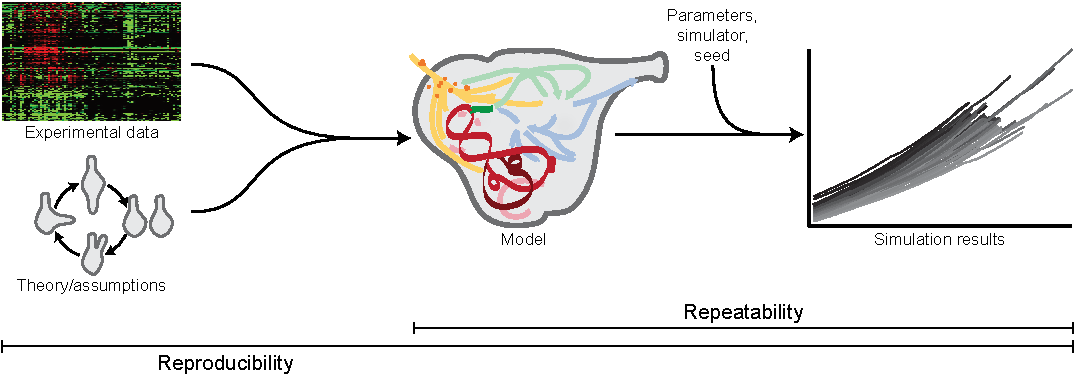
\includegraphics[width=\textwidth]{figure1/figure1}
% where an .eps filename suffix will be assumed under latex,
% and a .pdf suffix will be assumed for pdflatex; or what has been declared
% via \DeclareGraphicsExtensions.
\caption{Replicability and reproducibility explained: Model reproducibility refers to derivation from scientific knowledge and the ability to generate results in a reliable, repeatable manner;
Replicability refers only to the ability to recapitulate earlier simulation results}
\label{fig_repro_diagram}
\end{figure*}

\section{Replicability and Reproducibility}
Reproducing a model requires three steps (Fig.~\ref{fig_repro_diagram}). First, the model's equations and parameter values must be duplicated from the original assumptions and experimental data. This requires machine-readable standards for concretely describing model components in terms of external database entries such as KEGG \cite{kanehisa2000kegg} compounds and MetaCyc \cite{caspi2008metacyc} reactions, machine-readable databases for representing the data sources that were used to parameterize a model, annotation standards for describing how those data sources were used to parameterize the model, and annotation standards for describing the assumptions that the model was based on \cite{boulton2012open}. Such standards would also allow researchers to efficiently search and discover models.

Second, the model's numerical integrator must be duplicated. This requires that the simulation software source code be available and freely redistributable \cite{easterbrook2014open}.

Third, the numerical integrator must be used to duplicate the model's numerical results \cite{easterbrook2014open}. In the case of stochastic models, duplicating at least the first and second moments of the model's predictions is often used as a sufficient test of reproducibility. However, we argue that there are two advantages to reproducing the model's exact trajectory.

First, biology is replete with examples where rare events play key roles: e.g. cancer, speciation events, and mutations conferring antibiotic resistance. While these events may not occur often enough to contribute significantly to the expected dynamical behavior of a typical cell, they contribute significantly to the long-term behavior of the population. We believe that capturing these events when they occur will be instrumental to the usefullness of whole-cell models as engines for discovery and prevention of such rare events.

Second, being able to reproduce a trace of model timecourse behavior is absolutely crucial to scaling up to large and complex models. Human error has been and will continue to be a major source of inaccuracy in modeling experiments \cite{ebrahim2015genome}. The ability to reproduce an exact model trace would be highly useful in the context of model reproduction endeavors such as the workshop by Waltemath and Schreiber because this ability allows modelers to identify the exact point at which predictions diverge. Assuming such errors occur at a constant rate, a larger model would be expected to contain many more errors than a smaller one, and eliminating such costly errors is a prerequisite to the adoption of whole-cell modeling.

The idea of capturing the exact sequence of events leading to an error is not new. In the field of computer science, the SPIN model checker \cite{holzmann1997model} \cite{holzmann2004spin} has been used extensively to validate the operational logic of non-deterministic systems. SPIN detects invalid models by exhibiting a counterexample including the exact events leading to failure. We envisage a similar approach for biophysical modeling. Specifically, we envisage a simulator where not only can an exact simulation be replicated by supplying the same random seed, but also where a simulation may be restarted from a checkpoint containing a state snapshot at any point in the timecourse. Since serializing such checkpoints would be an expensive operation, the checkpoints would be user-specified. By combining these two features, we would be able to (1) replicate exactly a trace from a specific prior simulation, and (2) insert as many such checkpoints into the run as desired without affecting the outcome. We would then be able to capture rare events and apply permutations to test various hypotheses relating to the mechanism of the events, e.g. to test their robustness to knockouts and systematically screen for targets for intervention.

% In turn, to duplicate numerical results simulators should have complete deterministic control over their execution, including using deterministic algorithms and deterministic pseudorandom number generators. Chaotic models, which are highly sensitive to small numerical differences, and stochastic simulators, which cannot duplicate numerical results, are considerably more difficult to reproduce.

\subsection{Limitations of Current Standards for Reproducibile Modeling}

The CellML \cite{cuellar2003overview}, SBML \cite{hucka2003}, and SED-ML \cite{sedml2011} standards have greatly improved the replicability of dynamical modeling.
Despite these advances, many computational biology results still cannot easily be reproduced \cite{garijo2013quantifying}.

Part of this difficulty can be attributed to the gaps in the existing standards.
SBML helps researchers replicate model variables and equations and SED-ML helps researchers replicate simulation parameter values. 
However, neither standard helps researchers replicate simulators. 
In particular, neither standard ensures that simulators that use pseudorandom number generators can deterministically replicate stochastic simulation results, 
or that multiple simulators can replicate chaotic models.

A second barrier to reproducibility is the limited support for the existing standards.
One advantage of representing a model in a standard format such as SBML is the ability
to utilize multiple simulators to independently replicate simulation results. To support various specialized
modeling formalisms, SBML Level 3 includes several extensions including
Hierarchical Model Composition \cite{smith2015sbml},
Flux Balance Constraints\footnote{http://sbml.org/Documents/Specifications/SBML\_Level\_3/Packages/fbc}, and
Arrays\footnote{http://sbml.org/Documents/Specifications/SBML\_Level\_3/Packages/arrays} packages.
However, these packages have also fractioned SBML because each of these packages is only supported by a few simulators. 
In fact, no single simulator supports all of these packages.
This diminishes SBML's capability to facilitate replication.

A third barrier to reproducibility is the lack of transparency with respect to the experimental data and assumptions which models are based on.
This is becoming more important as researchers increasingly take advantage of high-throughput genomics data and pathway databases to build larger models.

\subsection{Technical Considerations for Replicability and Reproducibility}

Replicating a model is a useful step toward reproducing a model.
If a model's numerical simulations cannot be replicated, it will be
difficult to reproduce the model. Here, we discuss two technical issues which can 
cause non-replicable simulations -- concurrency and memory layout -- 
and approaches from computer science which have been successfully used to create 
deterministic software despite these issues.

Threading and asynchronous input/output callbacks execute instructions in an arbitrary,
non-deterministic order that is determined by a program's interaction with 
its operating environment. The increasing push to exploit multi-core CPUs has
led computer scientists to develop strategies for deterministically running software 
in a concurrent environment. Two systems that have been developed to eliminate non-determinism in threading
are C{\small ORE}D{\small ET} \cite{bergan2010coredet} and D{\small THREADS} \cite{liu2011dthreads}.
C{\small ORE}D{\small ET} is a framework and library for compiling C/C++ programs
such that the output executables behave deterministically, whereas
D{\small THREADS} is a replacement for the standard UNIX Pthreads library.
Both of these systems operate by preventing information sharing between
threads during a parallel phase, and deterministically allowing sharing
during a serial phase.
This biphasic structure imposes an overhead on the operation of the threading
system, but this overhead is low in many benchmarked cases \cite{liu2011dthreads}. 

These libraries also eliminate non-determinism
due to memory layout. D{\small THREADS} achieves this through a specially implemented memory allocator,
whereas C{\small ORE}D{\small ET} achieves this by compiling the
memory allocator itself with the C{\small ORE}D{\small ET} framework.

Some shortcomings of these tools include the fact that a small perturbation in initial
conditions can drastically affect program behavior.
Nevertheless, we believe that
dynamical modelers should use tools like C{\small ORE}D{\small ET} and D{\small THREADS}
to achieve replicable simulation algorithms, and that the systems biology community should
work toward producing software with robust determinism.

\subsection{Limitations of Current Standards for Whole-Cell Modeling}

The \textit{M. genitalium} whole-cell model \cite{Karr2012} consists of 28 submodels.
The submodels are implemented using a variety of modeling formalisms including
ordinary differential equations, Boolean networks, and flux balance analysis.

Although the \textit{M. genitalium} model is replicable, the model is not easily reproducible for several reasons. First,
although the model could be encoded in SBML using the Flux Balance Constraints, Hierarchical Model Composition \cite{smith2015sbml}, Multistate and Multicomponent
Species, and Array SBML packages, there is no SBML-compatible simulator which supports all of these packages or 
which can simulate multi-algorithm models. The existing SBML simulators only support 
model composition by flattening submodels into a single larger model. 

Second, the model is difficult to reproduce because the details of how experimental data was used to parameterize the \textit{M. genitalium}
are not transparent. The \textit{M. genitalium} model was parameterized using data from over 900 
sources. The WholeCellKB-MG database carefully describes these data sources \cite{karr2013wholecellkb}. Although this database is publicly accessible, 
the details of how this database was used to parameterize the model are unclear
because they are intertwined with the simulation code. 
Improved software tools must be developed to help whole-cell modelers use the minimum information 
requested in the annotation of biochemical models (MIRIAM) \cite{novere2005minimum}
standard to annotate model components with persistent uniform resource identifiers. 

Third, the model is difficult to reproduce because its assumptions are not clearly outlined. Rather, its assumptions are
implicit in the simulation source code. This makes it difficult
to distill the model's mathematical structure. A new standard is needed to allow modelers to annotate model assumptions, including why
specific mathematical formalisms were used and why those formalisms were appropriate. This standard should reference an ontology that 
includes common modeling assumptions.

Fourth, the model is difficult to reproduce because there is not yet a consensus multi-algorithm simulation meta-algorithm 
or consensus multi-algorithm simulation software system. An accurate, scalable multi-algorithm simulation meta-algorithm
and a high performance simulation program must be developed and accepted by the modeling community. This 
simulator must have deterministic control over its execution so that it can replicate 
simulations. In particular, it must have deterministic control over its use of pseudorandom number generators. 
In addition, multithreaded simulators should use libraries like C{\small ORE}D{\small ET} and D{\small THREADS} to 
ensure deterministic behavior on multi-core systems.

\subsection{Towards Hybrid Simulators}

The \textit{M. genitalium} was constructed from a limited set of data and its creators made carefully chosen compromises which reflect this fact. For example, metabolism is modeled using flux balance when a more detailed kinetic model could have been employed. Flux balance was chosen due to the fact that it does not require kinetic parameters in order to estimate the flux for a pathway, and it is difficult to obtain accurate values for these parameters in an organism such as \textit{M. genitalium}. We anticipate whole-cell models will continue to need to make such tradeoffs in the near future, so it follows that \texit{hybrid models} will become utilized more often in modeling studies.

A hybrid model employs diverse numerical solvers in calculating a timecourse trajectory. In general, these solvers will not be united by a common theoretical ground so it will not be possible to collapse (or ``flatten'') models into a single set of differential equations or rules which govern its dynamical behavior.
Instead, the dynamics will be derived from the internal behavior of the solvers and their interactions with each other. This allows modelers the freedom of choosing the optimum solver for a given role and availability of data.
Furthermore, 
% The utility of the model lies in providing optimal modeling of each of its subprocesses by choosing optimal modeling schemes on a case-by-case basis.
% Therefore, attempting to simplify or reduce the model would eliminate one of its most critical advantages. The disparate modeling techniques used in the model require different numerical solvers.

\section{Conclusion}

Expanded standards and new tools are needed to facilitate replicable and reproducible systems biology modeling, including whole-cell modeling.
These standards and tools must enable researchers to reproduce model assumptions, reproduce model parameters
directly from experimental data, and reproduce hybrid model simulations. 

One key step toward replicable modeling is expanded support for the 
Flux Balance Constraints, Hierarchical Model Composition \cite{smith2015sbml}, Multistate and Multicomponent
Species, and Array SBML packages. It is not necessary for every simulator
to support every package, but each simulator should be capable of numerically replicating its own results.
Consequently, each simulator must have deterministic control over its use of pseudorandom number generators.
New standards and tools to document model assumptions and data sources are also needed to enable researchers to reproduce models.
Such standards and tools will make it easier for independent researchers to understand, reproduce, and validate models. 
Finally, continued commitment to open standards, software tools, and models is needed to help researchers replicate and reproduce biologically accurate models.

\section{Acknowledgment}

The authors thank Herbert M. Sauro for helpful discussions
on reproducibility and replicability in systems biology.

% Can use something like this to put references on a page
% by themselves when using endfloat and the captionsoff option.
\ifCLASSOPTIONcaptionsoff
  \newpage
\fi

\bibliographystyle{IEEEtran}
\bibliography{IEEEabrv,model_reproducibility}

%%%%%%%%%%%%%%%%%%%%%
%% biography section
%%%%%%%%%%%%%%%%%%%%%
\begin{IEEEbiography}[{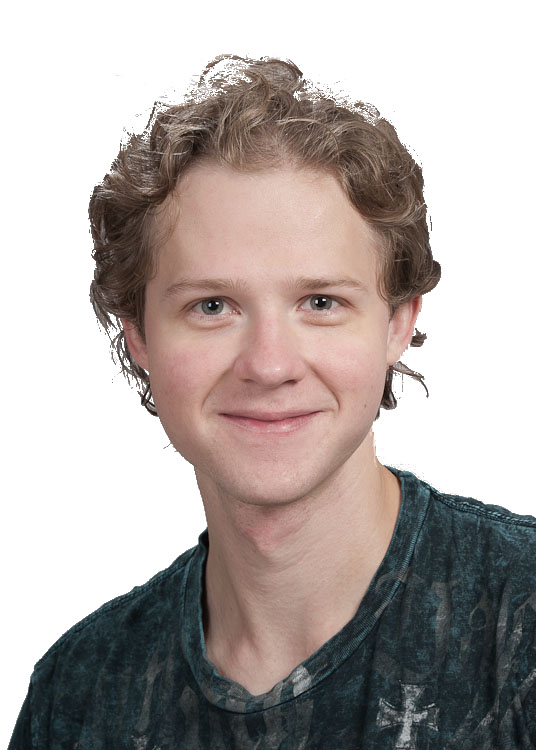
\includegraphics[width=1in,height=1.25in,clip,keepaspectratio]{photos/medley.jpg}}]{J. Kyle Medley}
obtained his BSc in Mechanical Engineering from the University of Missouri-Kansas City and
is currently pursuing a Ph.D. in Bioengineering from the University of Washington, USA.
His research interests include modeling dynamical biophysical processes such as
metabolism and gene expression regulation.
He currently develops libRoadRunner, a software package for simulating dynamical models encoded in SBML.
\end{IEEEbiography}

\begin{IEEEbiography}[{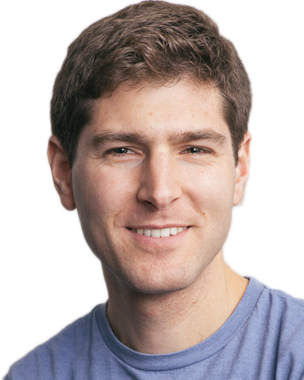
\includegraphics[width=1in,height=1.25in,clip,keepaspectratio]{photos/karr.jpg}}]{Jonathan R. Karr}
received his Ph.D. in Biophysics and M.S. in Medicine from Stanford University, USA in 2014 and his B.S.s in Physics and Brain \& Cognitive Sciences from the Massachusetts Institute of Technology, USA in 2006. Currently, Dr. Karr is a Fellow at the Icahn School of Medicine at Mount Sinai, USA. His research focuses on the development of comprehensive whole-cell computational models and their application to bioengineering and medicine.
\end{IEEEbiography}

\vfill

\end{document}